\documentclass[11pt]{scrartcl}
\usepackage[utf8]{inputenc} % Kodierung der Textdatei mit Sonderzeichen
\usepackage[ngerman]{babel} % Sprache fuer Inhaltsverzeichnis etc.
\usepackage{amssymb} % Mathematische Symbole
\usepackage{amsmath} % Mehr mathematische Konstrukte
\usepackage{graphicx} % Um Bilder einbinden zu koennen
\usepackage{float} % fuer \begin{figure}[H]
\usepackage{icomma} % laesst das Komma als Dezimaltrennzeichen interpretieren
\usepackage{fix-cm} % für die große Titelschrift
\usepackage[pdftex]{hyperref} % Hyperlinks im Dokument
\hypersetup{colorlinks=true, linkcolor=black, citecolor=black, filecolor=black, urlcolor=black, pdftitle={LED-Spektrometer - Projektpraktikum 09/10 Gruppe 5}}


\newcommand{\unit}[1]{\ensuremath{\,\mathrm{#1}}} % Einheiten schreiben sich immer aufrecht!
\newcommand{\degr}{\ensuremath{^\circ}}
\newcommand{\cel}{\ensuremath{\degr\mathrm{C}}}
\newcommand{\dif}{\ensuremath{\mathrm{d}}}
\newcommand{\pdif}[2]{\ensuremath{\frac{\partial#1}{\partial#2}}}
\newcommand{\ee}[1]{\ensuremath{\cdot 10^{#1}}}
\newcommand{\hypref}[2]{\hyperref[#2]{{#1}~\ref{#2}}}
\newcommand{\abb}[1]{\hyperref[#1]{Abb.~\ref{#1}}}
\newcommand{\tab}[1]{\hyperref[#1]{Tabelle~\ref{#1}}}

\setlength{\parindent}{1em}
\setlength{\parskip}{0.5\baselineskip}


\title{LED-Spektrometer - Gruppe 5 WS 09/10, Projektpraktikum der Uni Erlangen}
\date{07.12.2009 -- 15.01.2010}
\author{Michele Collodo, Andreas Glossner, Karl-Christoph G\"odel, Bastian Hacker, Maria Obst, Alexander Wagner, David Winnekens}



\begin{document}
\sloppy % laesst Latex nicht ueber den Rand rausschreiben
\thispagestyle{empty}
\large{Projektpraktikum WS 09/10}
\hfill
\raisebox{-1.4cm}{
\includegraphics[width=5cm]{images/fau.pdf}}
\\[8\baselineskip]
\begin{center}
{\fontsize{36}{54}\textbf{LED-Spektrometer}}
\\[2\baselineskip]
{\Large 07.12.2009 -- 15.01.2010}
\\[7\baselineskip]
{\huge\textbf{PPG 5}}
\\[0.5\baselineskip]
{\large\textbf{
Michele Collodo,
Andreas Glossner,\\
Karl-Christoph G\"odel,
Bastian Hacker,\\
Maria Obst,
Alexander Wagner,
David Winnekens}\\
Tutor: Xiaoyue Jin}
\vfill



\small{\url{http://pp.physik.uni-erlangen.de/groups/ws0910/ppg5/ppg5\_start.html}}
\end{center}
\newpage



\tableofcontents
\vfill



\begin{abstract}
Bla
\end{abstract}
\newpage


\section{Grundgedanke des Versuchs}

\subsection{Aufbau und Funktionsweise einer LED}
Die Leuchtdiode, kurz LED (für engl. "Light Emitting Diode") ist eine Halbleiter-Diode die es ermöglicht elektrische Energie in Licht verschiedener Wellenlängen umzuwandeln.\\
Da im vorliegenden Projekt nur bedrahtete LEDs als Absorber verwendet wurden, wird im Folgenden nur der Aufbau dieser Leuchtdioden-Bauform dargestellt. Die prinzipielle Funktionsweise ist jedoch bei fast allen Bauarten identisch. Lässt man durch Anode und Kathode der LED einen Strom in Durchlassrichtung fließen, so beginnt der Halbleiter in einer von Material und Dotierung abhängigen Wellenlänge zu strahlen. Für Leuchtdioden im sichtbaren Spektralbereich, wie sie hier verwendet wurden, kommt meist eine Galliumverbindung zum Einsatz.

\begin{figure}[ht]
\begin{center}
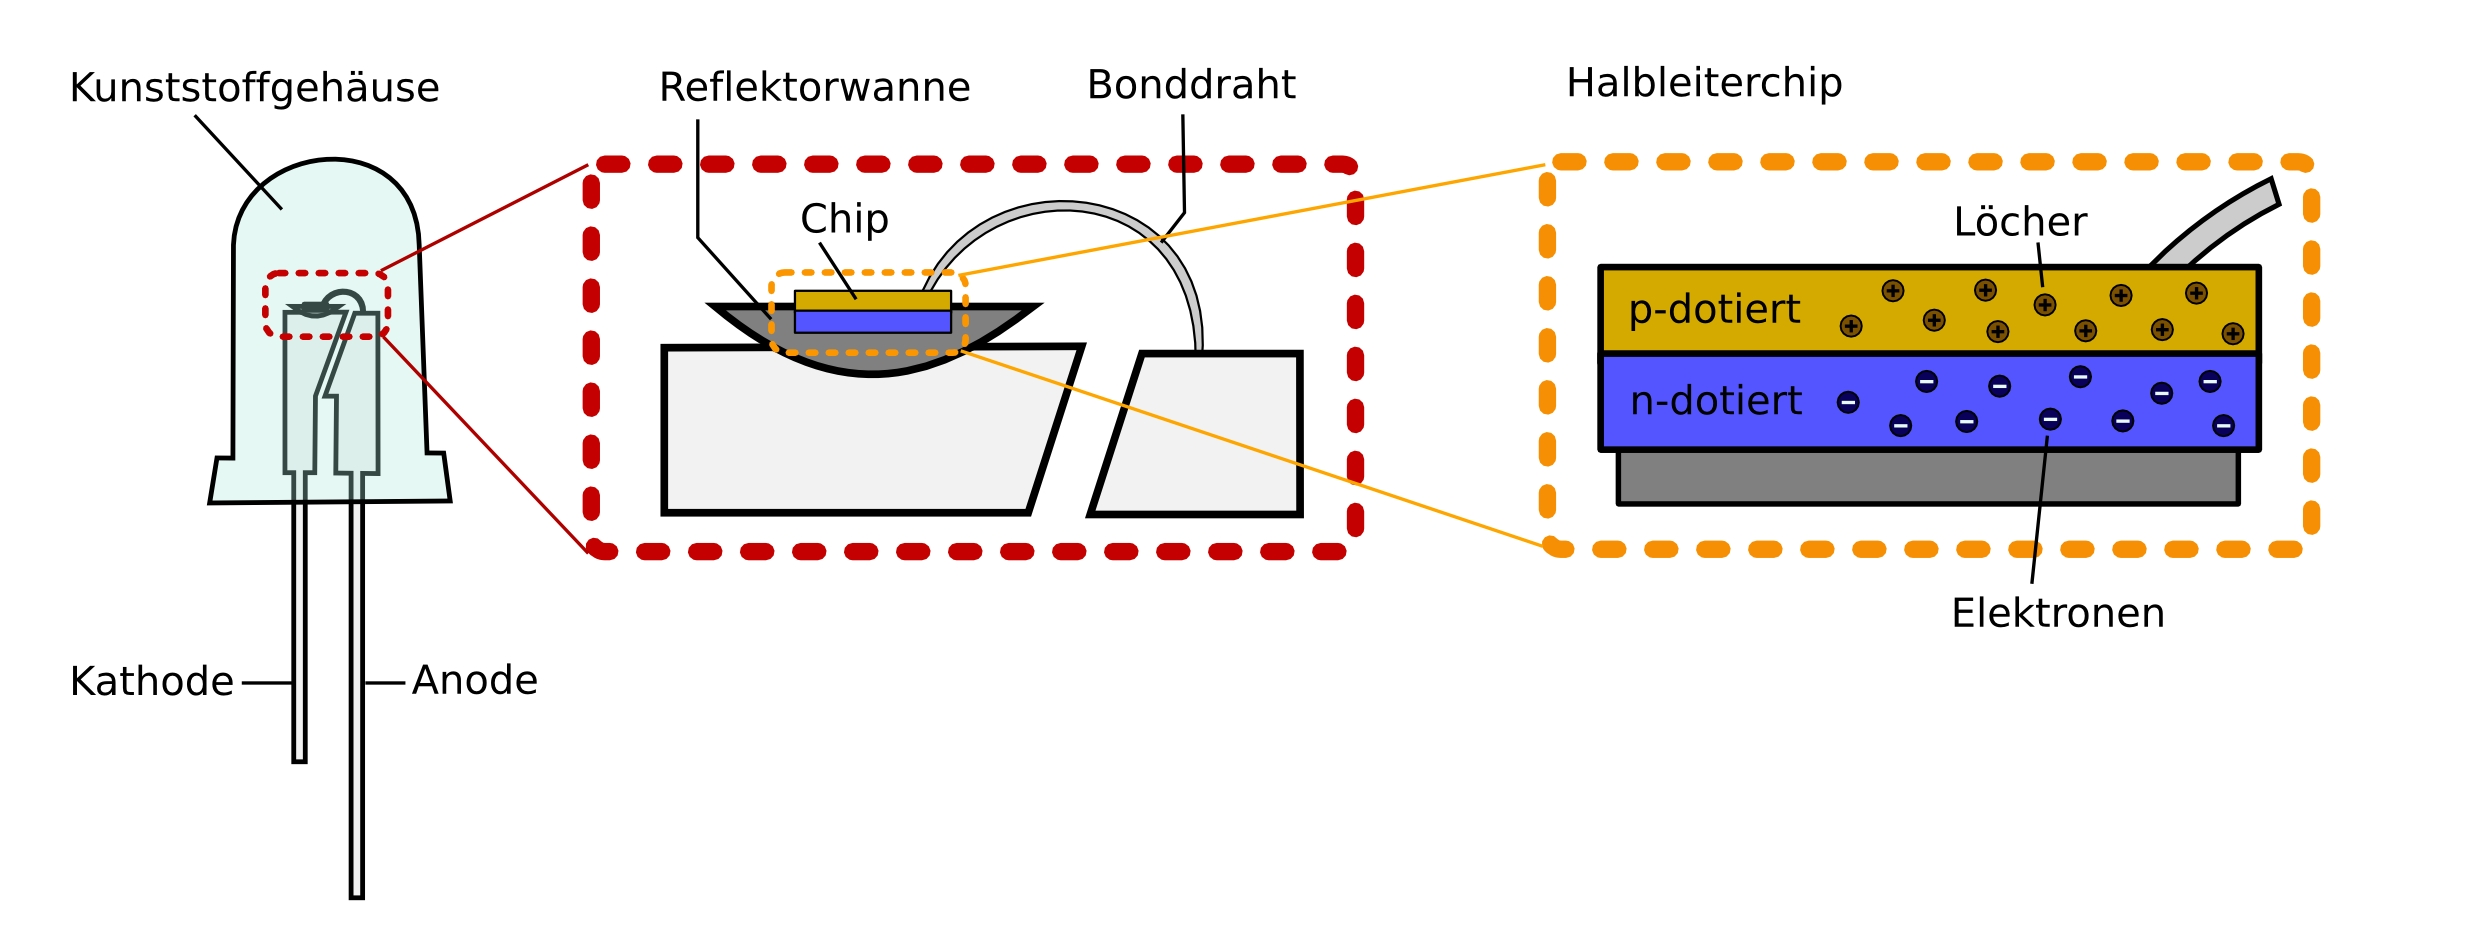
\includegraphics[width=0.8\textwidth]{images/ledaufbau.jpg}
\end{center}
\vspace{-1.5\baselineskip}
\caption{Aufbau einer bedrahteten Leuchtdiode}
\label{LED-Aufbau}
\end{figure}

Das Funktionsprinzip einer LED basiert auf dem Aufbau des Chips, der aus zwei verschieden dotierten Halbleiterschichten besteht. In der p-dotierten Schicht befindet sich ein Überschuss an positiven Ladungsträgern (Löcher), in der n-dotierten Schicht überwiegen negativ geladenen Teilchen (Elektronen). Wird nun ein Strom in Durchlassrichtung an den Chip angelegt, können Elektronen und Löcher am p-n-Übergang rekombinieren. Da sich die Elektronen im n-dotierten Halbleiter im Leitungsband befinden und auf das energetisch niedriger liegende Valenzband der p-dotierten Schicht wechsel, wo rekombinieren, wird ein fester Energiebetrag frei, der in Form eines Photons abgestrahlt wird.

\begin{figure}[ht]
\begin{center}
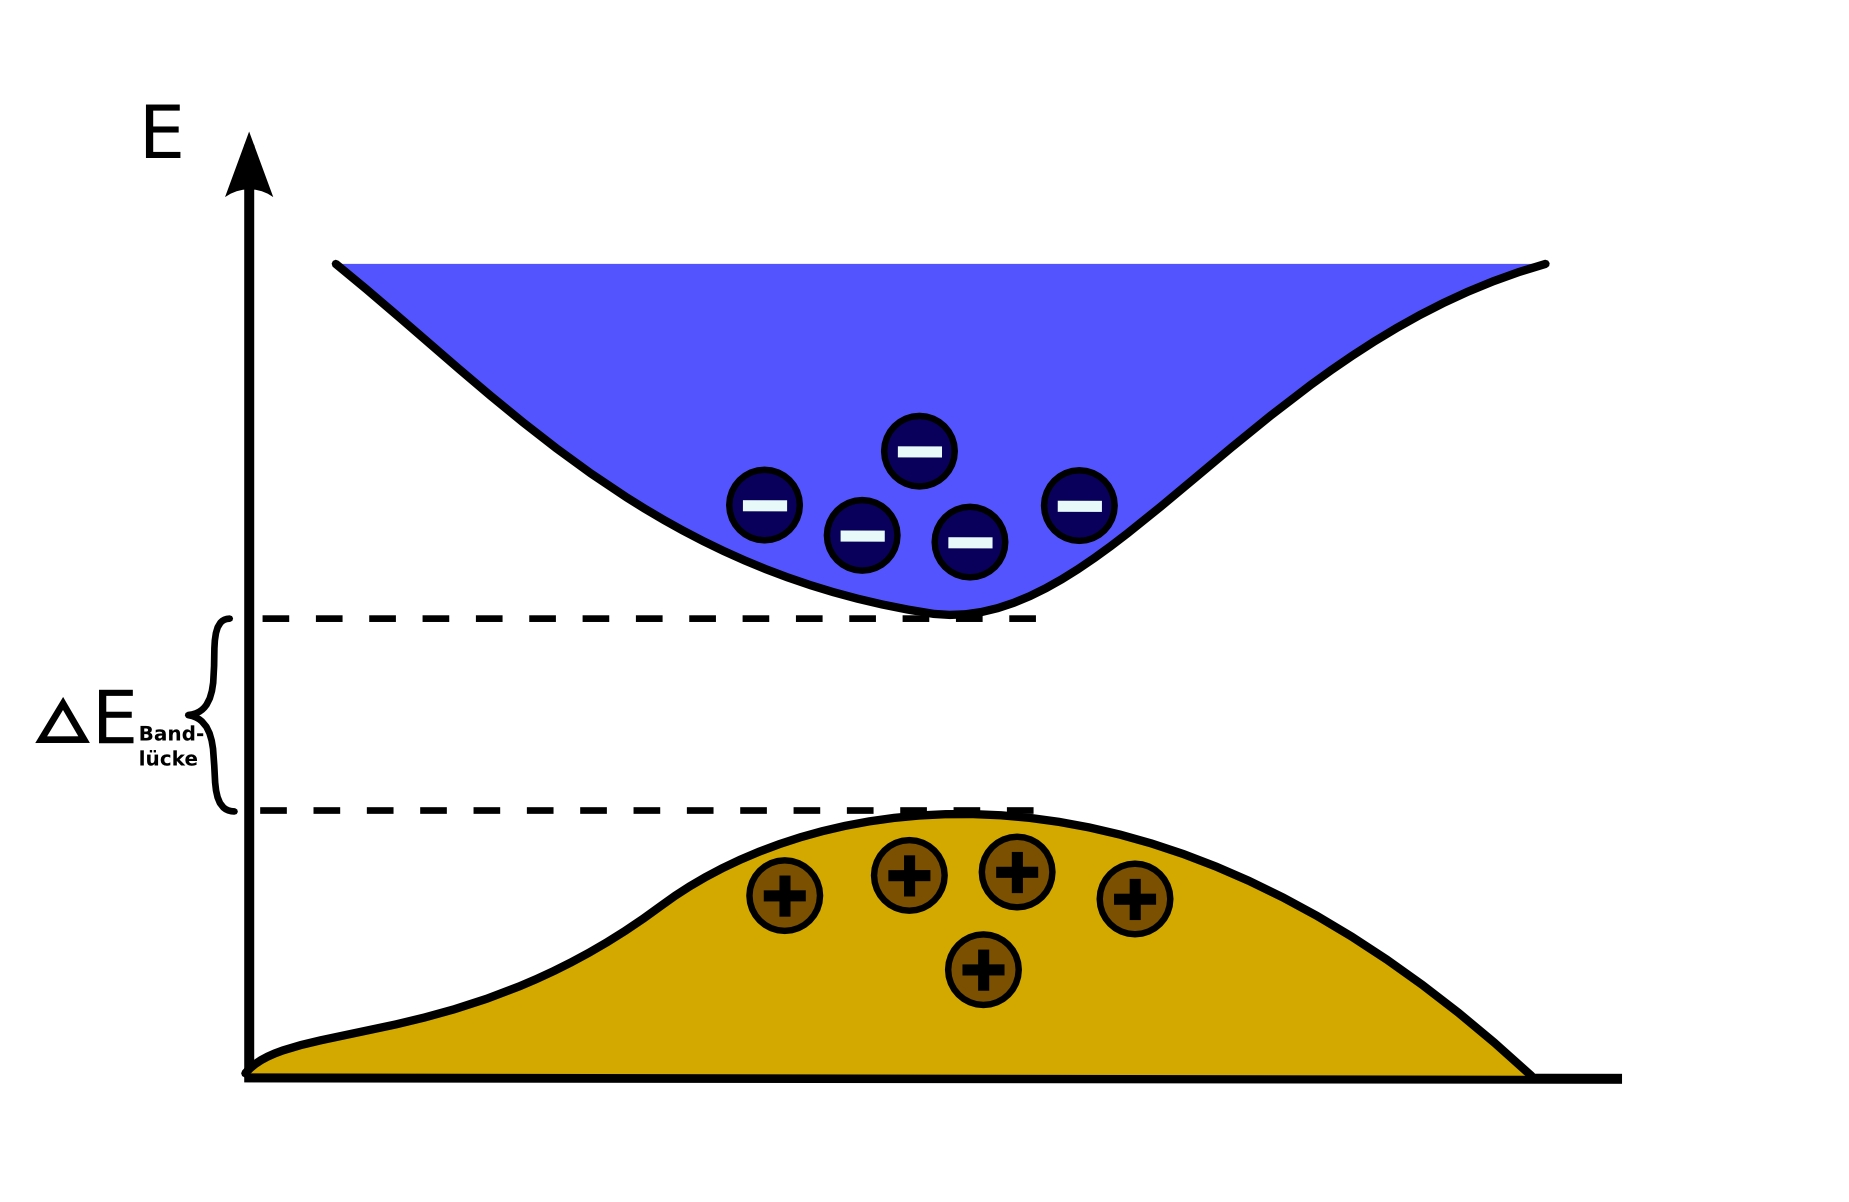
\includegraphics[width=0.8\textwidth]{images/band.jpg}
\end{center}
\vspace{-1.5\baselineskip}
\caption{Baenderstruktur der Halbleitergrenzschicht}
\label{Baendermodell}
\end{figure}

Die Energie dieses Photons entspricht der Bandlücke zwischen Valenzband und Leitungsband. Somit ergibt sich die Wellenlänge des emittierten Photons wie folgt:
 \[ \lambda = \frac{h \cdot c}{\Delta E_{Bandluecke}} \]
Dabei bezeichnet $h$ das Plancksche Wirkungsquatum und $c$ die Phasengeschwindigkeit des Lichts.

\subsection{Umkehrung des Effekts - LEDs in der Absorption}
In diesem Versuch sollten jedoch die LEDs nicht als Lichtemitter, sondern als Absorber dienen. Es wurde also versucht, die Funktionsweise der Lichtdioden umzukehren.\\
Bei Bestrahlung der LEDs mit Licht kann eine Spannung und ein Strom am Halbleiter abgegriffen werden. Besonderes Interesse gilt der Abhängigkeit dieses Stromes von der Wellenlänge des eingestrahlten Lichtes, je nach Farbe (Emissionswellenlänge) der LED. Da die Lichtdioden auch in der Absorption wellenlängenabhängig sind, ist es möglich aus mehreren Lichtdioden, die den gesamten visuellen Spektralbereich abdecken, ein Spektrometer für optische Spektren zu konstruieren.

\subsection{Vergleich von Emissions- und Absorptionsspektren}
Es stellt sich jedoch die Frage, wie Absorptions- und Emissionsspektrum der Leuchtdiode zusammenh\"angen.
Tr\"agt man Absorptions- und Emissionskurve in einem Diagramm auf, ist gut zu erkennen, dass das Absorptionsspektrum gegen\"uber der Emission blauverschoben ist. Die Verschiebung $\Delta \lambda$ ist jedoch bei verschiedenen LEDs unterschiedlich stark.

\begin{figure}[ht]
\begin{center}
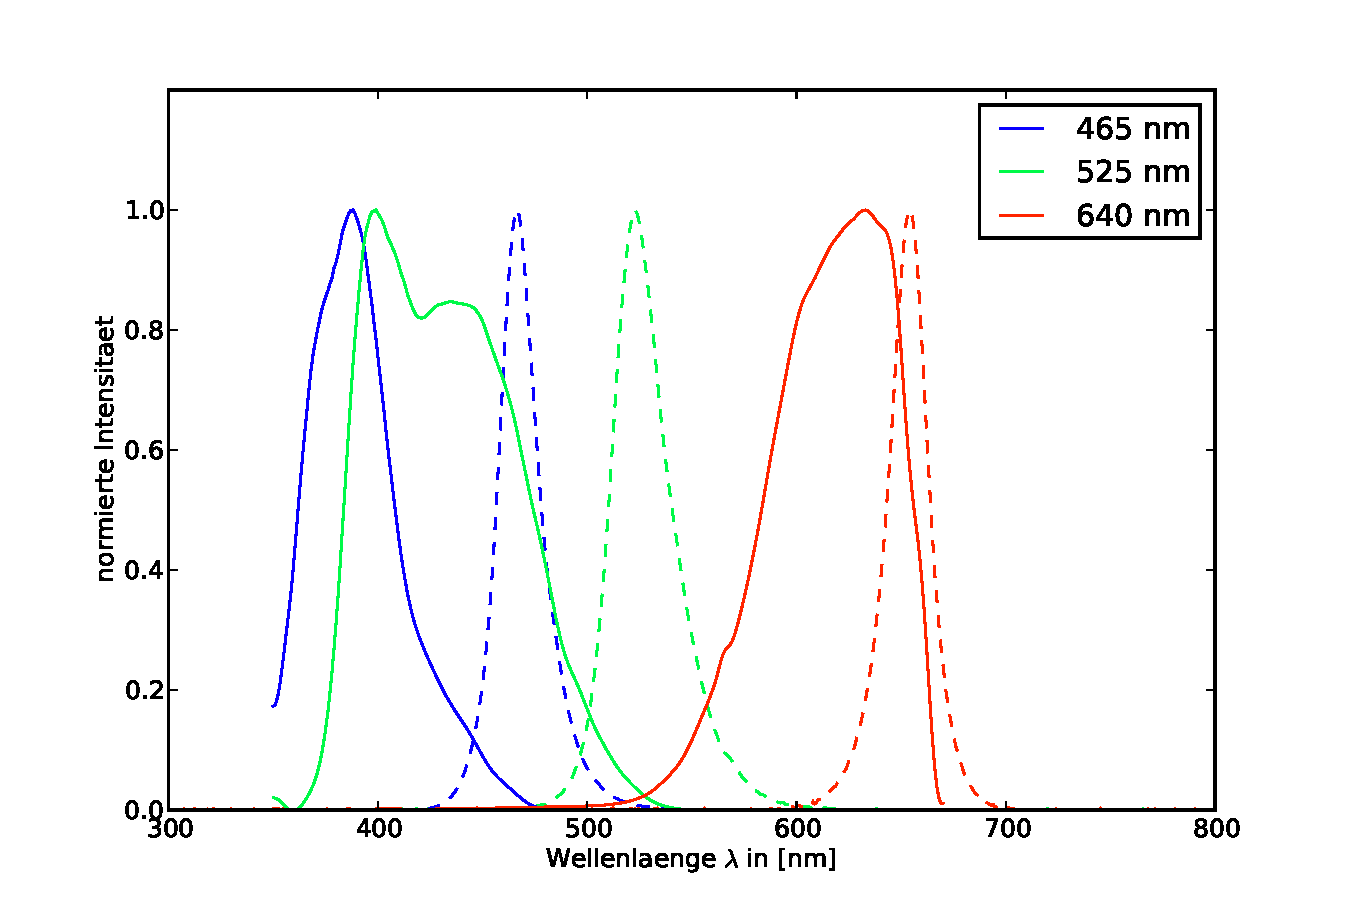
\includegraphics[width=0.9\textwidth]{images/absorp-emit.pdf}
\end{center}
\vspace{-1.5\baselineskip}
\caption{Absorptions- (durchgezogen) und Emissionsspektren (gestrichelt) verschiedener LEDs}
\label{Absorption und Emission von LEDs}
\end{figure}

%% Allg. was wir machen wollen, etwas Theorie 	Karl
%% Vergleich mit den Emissionsspekren}


\section{Messung der Absorptionsspektren}

\subsection{Versuchsaufbau}
%subsubsections wohl lieber weglassen, aber zur Meinungsbildung erst noch drinnen gelassen???	
\subsubsection{Lichtquelle} %%Axi
Die gew\"ahlte Lichtquelle sollte ein m\"oglichst breites Spektrum mit bekannter Intensit\"atsverteilung aufweisen. Da nur wenige verl\"a\ss{}liche Angaben bez\"uglich des jeweiligen Spektrums der Lampen zu finden waren, wurde beschlo\ss{}en das Spektrum der Lichtquelle mit einem entsprechenden Ger\"at im Institut f\"ur Optik zu ermitteln.\\
Zun\"achst wurde ein Verbund von 4 wei\ss{}en LEDs, die mit einem L\"ufter gek\"uhlt werden, als Lichtquelle f\"ur die Absorptionsmessung der sp\"ateren Mess-LEDs gew\"ahlt. Als Ergebnis der vier im Quadrat angeordneten LEDs wei\ss{}t deren aufgef\"achertes Spektrum waagrechte, dunkle Streifen auf, die von den Bereichen zwischen den LEDs stammen. Bei der Messung mu\ss{}te deshalb darauf geachtet werden, dass diese Zonen geringerer Intensit\"at zun\"achst durch Defokussieren des Aufbaus mithilfe der eingebauten Linsen verkleinert wurden und anschlie\ss{}end die LEDs die verbleibenden Streifen nicht kreuzen. Dies h\"atte entsprechende Verringerungen in der Intensit\"at des Absorptionsspektrums zur Folge, welche die Messdaten verf\"alschen w\"urden.\\
Bei der Auswertung wurde festgestellt, da\ss{} die erste Lichtquelle sehr wenig Intensit\"at im UV-Bereich emittiert. F\"ur die weiteren Messungen diente deshalb eine 50W Halogenlampe ohne UV-Filter als Lichtquelle. Diese zeigte st\"arkere Intensit\"at im UV-Bereich. Da die Halogenlampe mit etwas erh\"ohter Stromst\"arke betrieben wurde und Temperaturen um $200°C$ erreichen kann, war eine gute Bel\"uftung und ausreichender Abstand hitzeempfindlicher Teile auch hier wichtig.

\subsubsection{Strahlengang und Messaufbau} %%optischer Strahlengang ist unten eingebaut. Deshalb auch die Idee, die subsubsections weg zu lassen.
Zur Erzeugung eines Spektrums gibt es diverse M\"oglichkeiten. Es stellte sich aber heraus, dass die Verwendung eines Prismas aufgrund der geringen Winkelausdehnung des erzeugten Spektrums f\"ur uns wenig lohnenswert ist. Ebenso mussten wir trotz langen Experimentierens und unter Verwendung verschiedener Linsenanordnungen auch auf ein Transmissionsgitter verzichten, da die Intensit\"at des Spektrums nicht stark genug war. Folglich griffen wir auf ein holographisches Reflexionsgitter zur\"uck.\\%%Gitterkonstante und Winkelausdehnung des Spektrums angeben
%%\subsubsection{Winkelmessung} %%--- Eher "Wellenl\"angenbestimmung" oder dergleichen?! Da wir dadurch ja die momentan gemessene Wellenl\"ange bestimmen m\"ochten
F\"ur die Auswertung der Messdaten ist es von grundlegender Bedeutung, zu wissen welcher Wellenl\"ange die gemessene Intensit\"at zuzuordnen ist. Um dies zu erreichen wurde folgendes Vorgehen gew\"ahlt: Durch die Verwendung eines Refelxionsgitters und dessen Justierung derart, dass der Strahlengang in einer zum optischen Tisch parallelen Ebene verl\"auft, l\"asst sich die Wellenl\"ange durch Formel XXX leicht in den Winkel zwischen ein- und ausfallendem Strahl umrechnen. Da ein manuelles Auslesen der Intensit\"at und dessen zugeh\"origem Winkel ein aussichtsloses Unterfangen darstellen w\"urde, benutzten wir ein Drehpotentiometer zur automatischen Auswertung des momentanen Winkels. Dieses wurde so auf dem Tisch positioniert, dass die Drehachse m\"oglichst genau unter dem Mittelpunkt des Gitters ist, also dem Punkt, an welchem sich ein- und ausfallender Strahl treffen. Desweiteren wurde der Dreharm, an dessen \"Au\ss{}erstem Ende sich der Halter f\"ur die LEDs befindet, mit der Drehachse verbunden, sodass das Schwenken des Armes den Widerstand des Potentiometeres \"andert.

\begin{figure}[ht]
\begin{center}
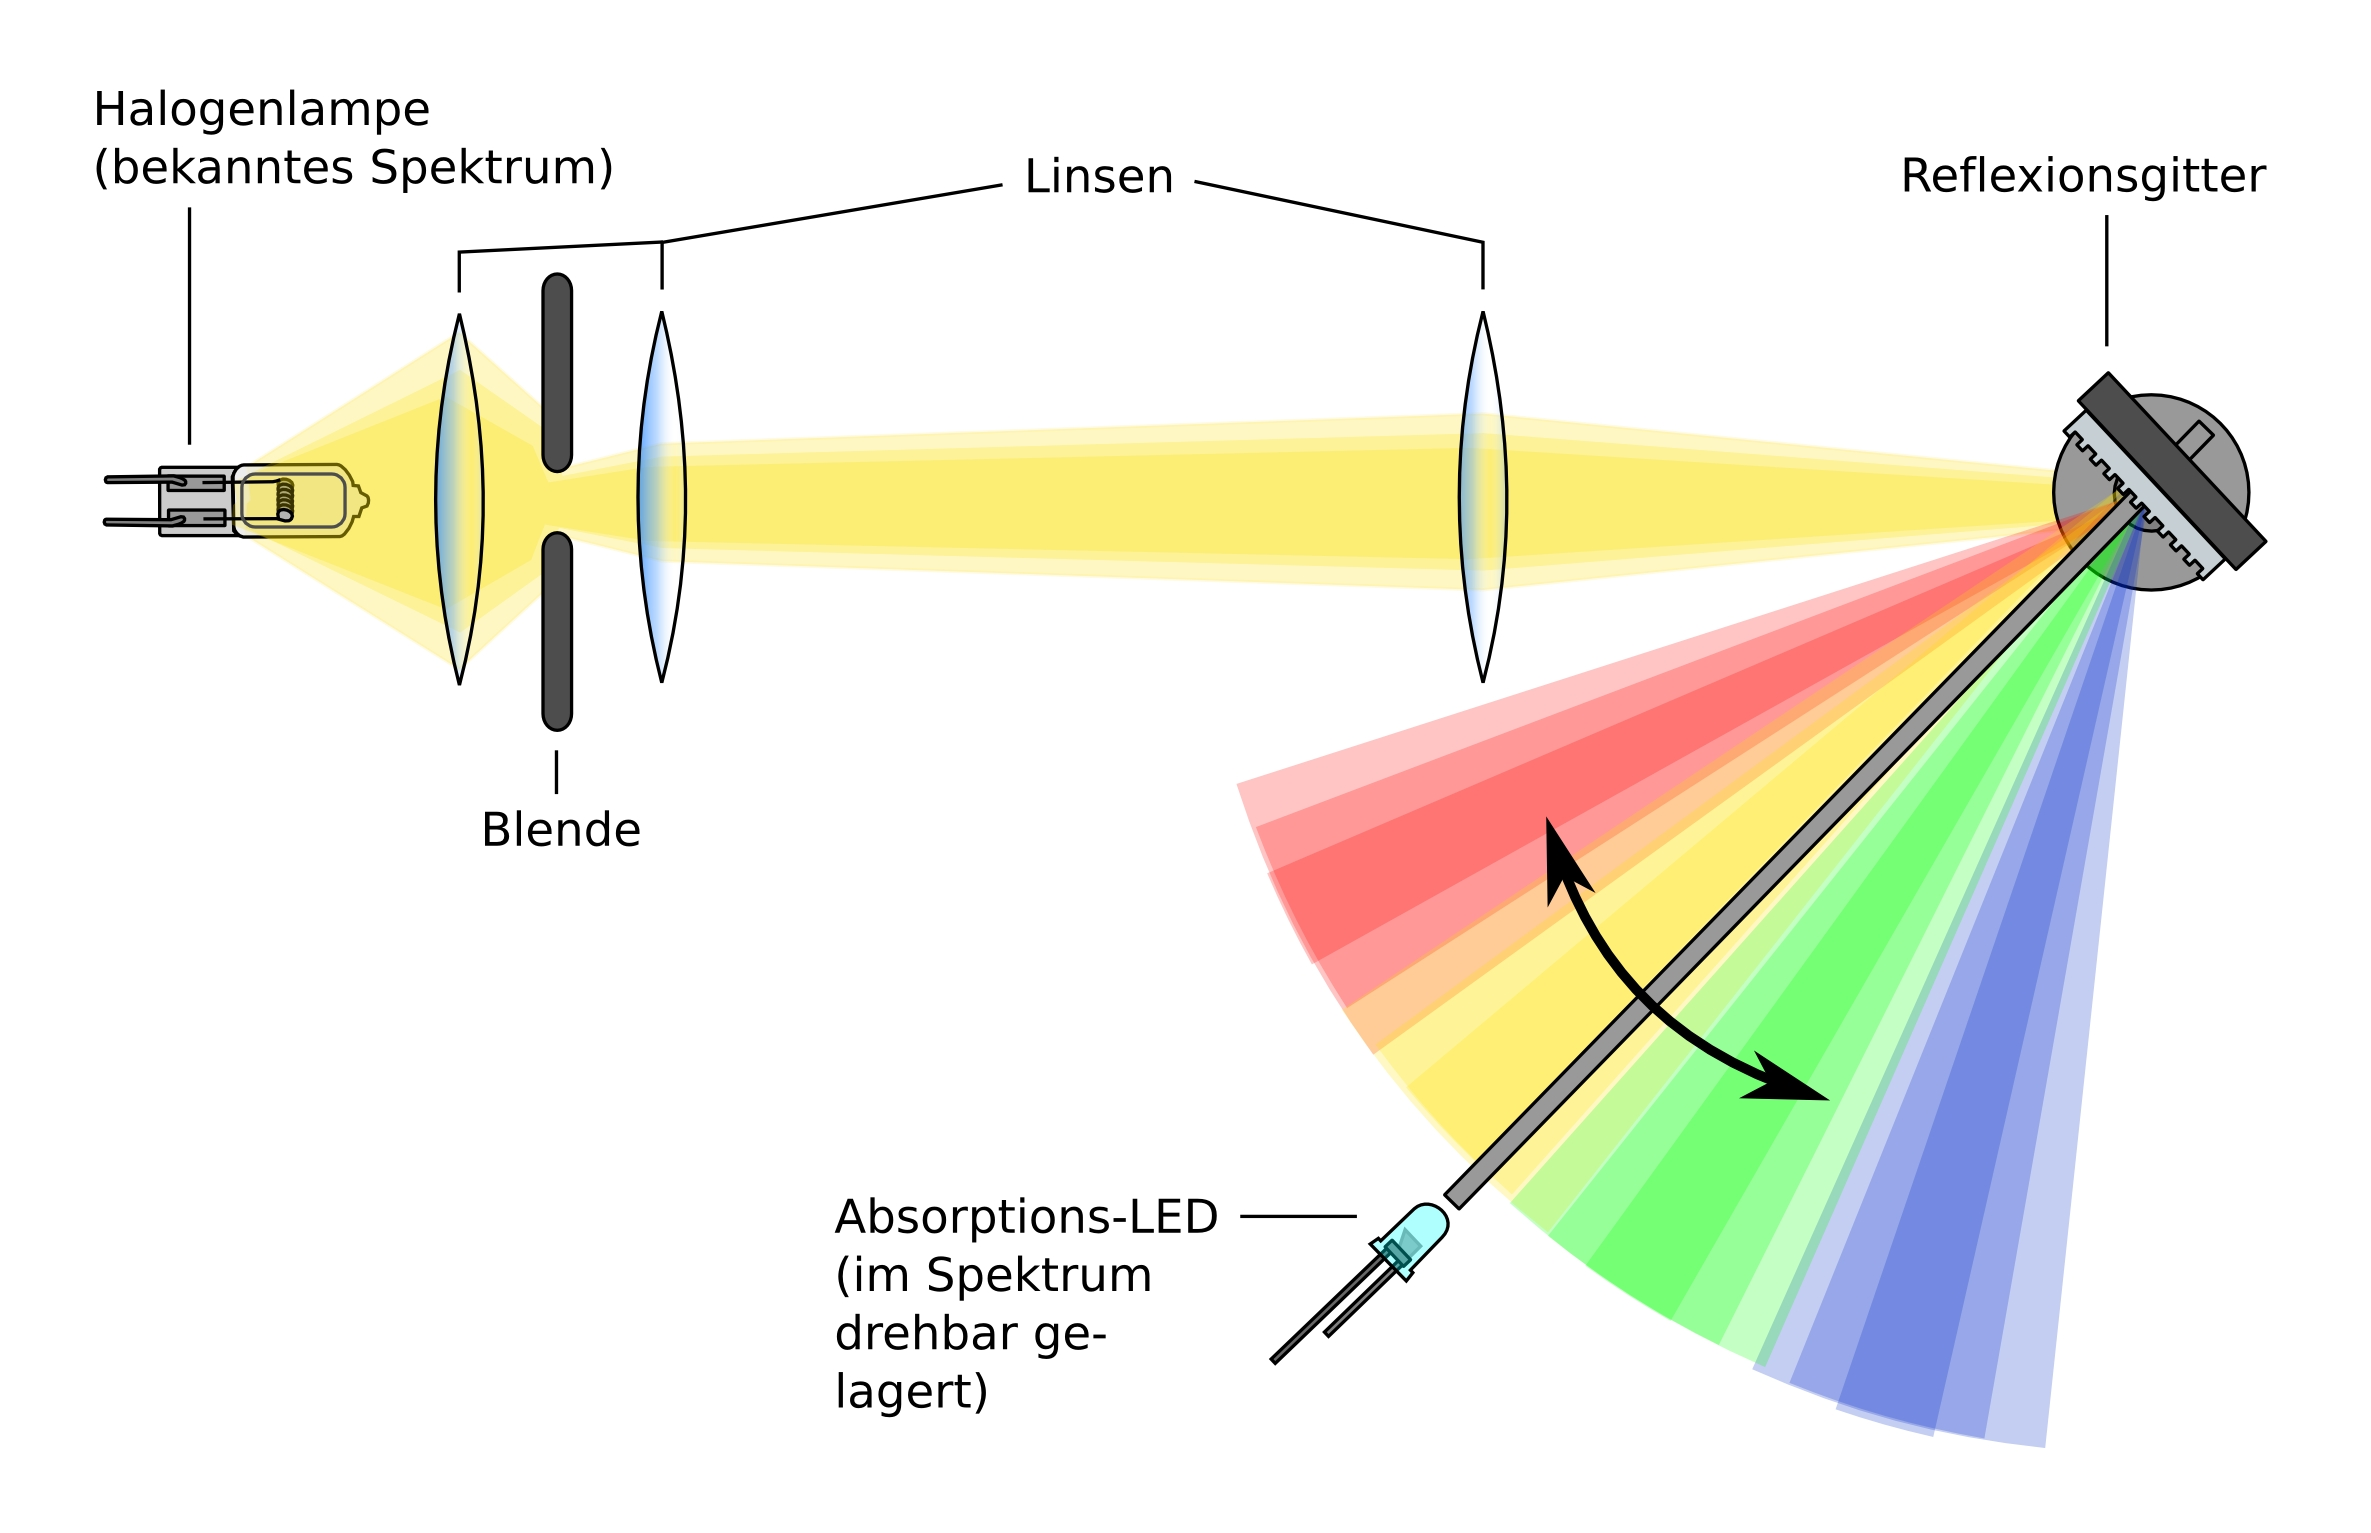
\includegraphics[width=0.8\textwidth]{images/setup.jpg}
\end{center}
\vspace{-1.5\baselineskip}
\caption{Versuchsaufbau}
\label{Versuchsaufbau}
\end{figure}

Anschließen wurde in $2^\circ$-Intervallen der Winkel und die Spannung am Potentiometer notiert. Wiederholtes Messen dieser Spannungs-Winkel-Abhängigkeit zeigte eine sehr gut Reproduzierbarkeit. Lediglich beim Wechsel des Drehsinns zeigte sich ein Offset, sodass entschlossen wurde alle Messungen immer mit Drehung im Uhrzeigersinn durchzuführen.\\
Somit konnten wir die momentane Spannung am Potentiometer auslesen lassen, was uns den Winkel gibt und somit die Wellenlänge berechnen lässt.


\subsection{Reduktion der Spektren}
%% Fit der Winkelfunktion
%% Entfaltung                 Basti





\section{Bau des Spektrometers}
\subsection{Funktionsprinzip Übersicht}

\subsection{Elektronik}
%% Funktionsprinzip OpAmps etc.			Michele, Maria
%% Schaltplan

\subsection{Auswertungsprogramm}
% Software: Berechnung der Spektren mit unserem Gerät
%% Funktionsübersicht und Erklärung der Bedienung
%% Algorithmik zur Auswertung					BAsti



\newpage
\section{Autorenverzeichnis}
\begin{tabular}{|l|l|}
\hline
\emph{Autor} & \emph{Kapitel}\\
\hline
Michele Collodo & \\
Andreas Glossner & \\
Karl-Christoph G\"odel & \\
Bastian Hacker & \\
Maria Obst & \\
Alexander Wagner & \\
David Winnekens &  \\
Wickie Pedia & Recherchen \\
\hline
\end{tabular}
\end{document}

